
%% The first command in your LaTeX source must be the \documentclass command.
\documentclass[sigconf,authordraft]{acmart}

%% ==========================================
%% PACKAGES & CUSTOM DEFINITIONS
%% ==========================================
\usepackage{enumitem}
\usepackage{multirow}
\usepackage{graphicx}
\usepackage{xcolor}
\usepackage{tikz}
\usetikzlibrary{arrows.meta,positioning}

% Define Colors for Each Reviewer (Matching the image style)
\definecolor{revVY3D}{RGB}{34, 139, 34}   % Green
\definecolor{revjV7P}{RGB}{0, 0, 255}     % Blue
\definecolor{revhrcD}{RGB}{255, 20, 147}  % Magenta
\definecolor{revuUZG}{RGB}{210, 105, 30}  % Orange
\definecolor{revovZo}{RGB}{148, 0, 211}   % Purple

% Global Formatting adjustments for space saving in 1-page limit
\setlist[enumerate]{leftmargin=*,nosep}
\setlist[itemize]{leftmargin=*,nosep}
\setlength{\parindent}{0pt}
\setlength{\parskip}{0.4em}

% Custom Rebuttal Commands (Styled like the provided image)
\newcommand{\revheader}[3]{
    \vspace{1em}
    \begin{center}
        \textbf{\color{#1} \rule{0.15\linewidth}{0.7pt}\quad To Reviewer #2 (#3) \quad\rule{0.15\linewidth}{0.7pt}}
    \end{center}
    \vspace{-0.5em}
}

\newcommand{\question}[3]{
    \vspace{0.4em}
    \noindent\textbf{\color{#1}#2} #3
}

\newenvironment{answer}{
    \vspace{0.2em}
}{
    \vspace{0.6em}
}

%%
%% \BibTeX command to typeset BibTeX logo in the docs
\AtBeginDocument{%
  \providecommand\BibTeX{{%
    \normalfont B\kern-0.5em{\scshape i\kern-0.25em b}\kern-0.8em\TeX}}}

\settopmatter{printacmref=false} % Removes citation information below abstract
\renewcommand\footnotetextcopyrightpermission[1]{} % removes footnote with conference information in first column
\pagestyle{empty} % removes running headers 
\setcopyright{none}

\begin{document}

%% ==========================================
%% ANONYMOUS DOCUMENT METADATA (Double-Blind Compliant)
%% ==========================================
\title{Author Rebuttal for Paper \#4778}

\maketitle
\thispagestyle{empty}

% ==========================================
% GENERAL RESPONSE / CONSOLIDATED SUMMARY
% ==========================================
We appreciate all reviewers' recognition and valuable suggestions. We address the specific concerns raised by each reviewer below.
% ==========================================
% REVIEWER VY3D 
% ==========================================
\vspace{-5mm}
\revheader{revVY3D}{VY3D}{Rating: 3}
\vspace{-2mm}
\question{revVY3D}{VY3D-Q1: Explanation of Baseline Performance.}{}
\begin{answer}
    \vspace{-4mm}
    \begin{figure}[h]
    \centering
    % \vspace{-2mm}
    \resizebox{\linewidth}{!}{%
    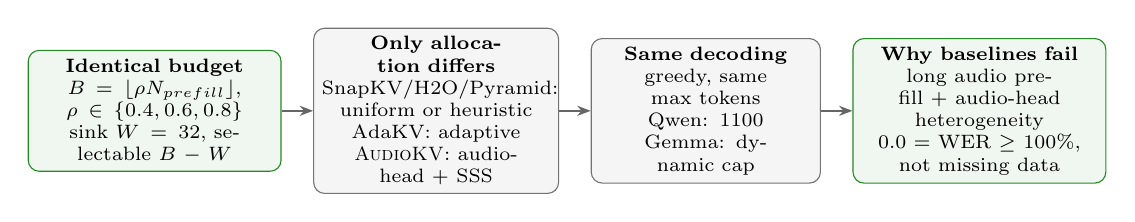
\begin{tikzpicture}[
        node distance=4mm,
        box/.style={draw, rounded corners, align=center, inner sep=3pt, minimum height=8mm, font=\scriptsize},
        greenbox/.style={box, draw=revVY3D, fill=revVY3D!7},
        graybox/.style={box, draw=black!55, fill=black!4},
        arr/.style={-{Stealth[length=1.7mm]}, thick, draw=black!60}
    ]
        \node[greenbox, text width=30mm] (budget) {\textbf{Identical budget}\\$B=\lfloor\rho N_{\text{prefill}}\rfloor$, $\rho\in\{0.4,0.6,0.8\}$\\sink $W=32$, selectable $B-W$};
        \node[graybox, text width=29mm, right=of budget] (alloc) {\textbf{Only allocation differs}\\SnapKV/H2O/Pyramid: uniform or heuristic\\AdaKV: adaptive\\\textsc{AudioKV}: audio-head + SSS};
        \node[graybox, text width=27mm, right=of alloc] (decode) {\textbf{Same decoding}\\greedy, same max tokens\\Qwen: 1100\\Gemma: dynamic cap};
        \node[greenbox, text width=30mm, right=of decode] (failure) {\textbf{Why baselines fail}\\long audio prefill + audio-head heterogeneity\\0.0 = WER $\geq$ 100\%, not missing data};
        \draw[arr] (budget) -- (alloc);
        \draw[arr] (alloc) -- (decode);
        \draw[arr] (decode) -- (failure);
    \end{tikzpicture}%
    }
    \vspace{-4mm}
    \vspace{-5mm}
    \end{figure}
    
    Under this matched setting, every method uses the same dynamic prefill budget $B$, sink window, and decoding horizon; the retention ratio changes only the prefill cache size, so Table~1 isolates the allocation strategy not giving \textsc{AudioKV} extra memory or decoding steps. The near-zero baseline scores therefore reflect a long-form audio domain shift: longer prefill sequences and heterogeneous audio-critical heads make text-oriented eviction unstable, causing repetition collapse where bounded word accuracy becomes 0.0.
\end{answer}

 \vspace{-5mm}
\question{revVY3D}{VY3D-Q2: Computational Overhead.}
\vspace{-1mm}
    We added an end-to-end wall-clock timing comparison with identical model weights, input samples, decoding configuration, and KV budget, changing only whether SSS is enabled.
    \vspace{-3mm}
    \begin{table}[h]
    \centering
    \resizebox{\linewidth}{!}{%
    \begin{tabular}{lccc}
    \toprule
    \textbf{Metric} & \textbf{SSS disabled} & \textbf{SSS enabled} & \textbf{Change} \\
    \midrule
    Avg. audio duration / sample & 190.80s & 190.80s & -- \\
    Avg. wall time / sample & 22.2139s & 22.3830s & +0.1691s (+0.76\%) \\
    Real-time factor (RTF) & 0.11642 & 0.11731 & +0.76\% \\
    End-to-end output throughput & 26.32 tok/s & 26.13 tok/s & -0.73\% \\
    \bottomrule
    \end{tabular}%
    }
    \end{table}
    \vspace{-5mm}
    The measured delta is within normal run-to-run variation. SSS adds no material end-to-end latency penalty in this setting while preserving the KV-cache reduction.


\vspace{-3mm}
\question{revVY3D}{VY3D-Q3: Source of Head Importance.}
\vspace{-1mm}
To isolate the impact of \emph{audio-aware supervision} in SSS, we evaluate three head-importance sources (audio-aware, inverse, random with seed 42) on Qwen2.5-Omni-3B (left) and Gemma-3n-E4B-it (right). All variants use a budget of $\rho=0.8$ on 20\% MLS ASR subsets; lower WER is better.

\vspace{-4mm}
\begin{figure}[h]
\centering
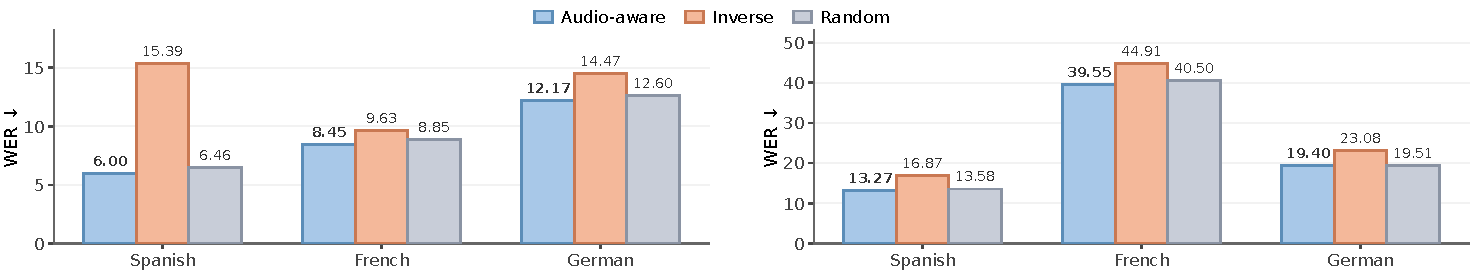
\includegraphics[width=\linewidth]{figures/vy3d_q3_audio_supervision_subplots.pdf}
\vspace{-2mm}
\end{figure}

\vspace{-6mm}
The audio-aware head prior consistently outperforms other variants across all six MLS ASR settings, particularly in Spanish. Overall performance follows the order of \text{audio-aware} > \text{random} > \text{inverse}, confirming that audio-aware supervision is essential for downstream tasks requiring acoustic evidence preservation.


% ==========================================
% REVIEWER jV7P 
% ==========================================
\vspace{-5mm}
\revheader{revjV7P}{jV7P}{Rating: 4}
\vspace{-2mm}
\question{revjV7P}{jV7P-Q1: Offline Head Profiling Dataset.}
We agree that the head-importance scores and the resulting budget-allocation policy depend on the offline calibration corpus. In our experiments, we use the LibriSpeech \texttt{test-other} split as the offline profiling dataset, which contains 2,605 successfully profiled utterances. This corpus covers only standard English read speech and is strictly disjoint from our main LibriSpeech evaluation, as the results in Table~1 are evaluated on the \texttt{test-clean} split, ensuring no overlap.

\vspace{-3mm}
\question{revjV7P}{jV7P-Q2: Comparison to Simpler Smoothers.}{There is no comparison to simpler smoothers that would isolate whether frequency-domain filtering specifically is doing the work.}
We added a controlled smoother ablation on Qwen2.5-Omni-3B with budget $\rho=0.4$, keeping SparseKV and head scores fixed while changing only the score smoother.
We report completed 20\% MLS ASR subsets for Spanish (477), French (486), and German (679 utterances).

\vspace{-3mm}
\begin{table}[h]
\centering
\vspace{-3mm}
\resizebox{\linewidth}{!}{%
\begin{tabular}{lcccccc}
\toprule
\textbf{Task (WER $\downarrow$)} & \textbf{None} & \textbf{MaxPool} & \textbf{Gaussian} & \textbf{Uni-stride} & \textbf{Uni-prior} & \textbf{SSS} \\
\midrule
MLS Spanish (477) & 890.61 & 890.61 & 890.61 & 890.61 & 890.61 & \textbf{31.52} \\
MLS French (486) & 747.97 & 747.97 & 747.97 & 747.97 & 747.97 & \textbf{24.90} \\
MLS German (679) & 1417.18 & 1417.18 & 1417.18 & 1417.18 & 1417.18 & \textbf{60.28} \\
\bottomrule
\end{tabular}%
}
\end{table}

\vspace{-3mm}
Across Spanish, French, and German, non-spectral smoothers all trigger repetitive decoding collapse, whereas SSS restores stable generation (SSS WER: 31.52/24.90/60.28; long decodes $\ge 1000$ tokens: 5/477, 2/486, 10/679).
The benefit is therefore not explained by smoothing in general; frequency-domain filtering is specifically vital for stable cache selection under the same low budget.


% ==========================================
% REVIEWER hrcD 
% ==========================================
\vspace{-5mm}
\revheader{revhrcD}{hrcD}{Rating: 5}
\vspace{-2mm}
\question{revhrcD}{hrcD-Q5: Cross-Task Discrepancies in Baseline Failure.}
\vspace{-1mm}
The discrepancy stems from \textit{generation horizon} and \textit{metric sensitivity}. Long-form autoregressive tasks like ASR/ST require extended decoding steps where mid-generation context loss heavily triggers self-reinforcing repetition loops, whereas AQA benchmarks generate short answers with fewer steps for token-level degradation to snowball. Furthermore, ASR uses rigid sequence-alignment metrics (WER) that penalize structural faults severely, while AQA utilizes an \textit{LLM-as-a-Judge} framework that tolerates minor stylistic degradations as long as the core entity is preserved.


% ==========================================
% REVIEWER uUZG 
% ==========================================
\vspace{-5mm}
\revheader{revuUZG}{uUZG}{Rating: 4} 

\vspace{-2mm}
\question{revuUZG}{uUZG-Q1: Sensitivity to Alignment Data.}
The identified audio-critical attention heads capture the model's intrinsic modality bias formed during pre-training, rather than artifacts from profiling data. Our experiments prove cross-lingual and cross-task generalization: despite profiling on English ASR, the allocation policy achieves near-full accuracy zero-shot on Mandarin, European languages, and four distinct downstream Audio QA tasks. Furthermore, Spectral Score Smoothing (SSS) acts as a global frequency-domain regularizer, mitigating minor sub-optimality caused by domain shifts.

\vspace{-2mm}
\question{revuUZG}{uUZG-Q4: Orthogonal Quantization Approaches.}{Discussing or evaluating orthogonal compression (eviction + quantization) would strengthen the contribution.}
KV eviction and KV quantization (e.g., KIVI) are fundamentally orthogonal efficiency techniques. AudioKV dynamically evicts non-essential tokens globally, and KIVI can subsequently quantize the preserved KV pairs. Exploring this joint compression represents a highly promising direction for real-world deployment on resource-constrained devices.


% ==========================================
% REVIEWER ovZo 
% ==========================================
\vspace{-5mm}
\revheader{revovZo}{ovZo}{Rating: 3}

\vspace{-2mm}
\question{revovZo}{ovZo-Q1: Novelty Boundary Against SparseMM.}
We agree that the head-importance scores and the resulting budget-allocation policy depend on the offline calibration corpus. Specifically, our calibration dataset is LibriSpeech (\texttt{test-other} split, containing 2,605 successfully profiled utterances), covering English read speech only. Furthermore, this corpus is disjoint from our main LibriSpeech evaluation: Table~1 LibriSpeech results use \texttt{test-clean}, ensuring that the profiling corpus does not overlap with the evaluation set.


\vspace{-3mm}
\question{revovZo}{ovZo-Q5: Clarification of 0.0 Failure Entries.}{The 0.0 entries and metric handling in Table 1 need clearer explanation.}
In the revision, we will clarify that Table~1 reports bounded task accuracy:
$ \mathrm{Acc}_{\mathrm{WER}}=\max(0, 100-\mathrm{WER})$.
A 0.0 means the raw error rate reached or exceeded 100\% (e.g., severe insertion-heavy prefix hallucinations or repetition loops). It does \emph{not} mean the sample was skipped or that the generated output was completely blank.

\end{document}
